\chapter{Results}

\section{Annotation Statistics}

Concepts in the annotations appear appropriate for a typical textual corpus. Figures \ref{fig:idf-scores} and \ref{fig:tf-scores} are what one would expect to see; that is, the distribution is Zipfian~\cite{tullo2003modelling}. Each figure displays 40 of the 2041 terms and concepts in total. Note that the notion of concepts are different to terms since a concept can contain more than once word (this is possible through tags, where a tag can contain multiple words such as `shopping mall' and `street sign').

\begin{figure}[!ht]
    \centering
    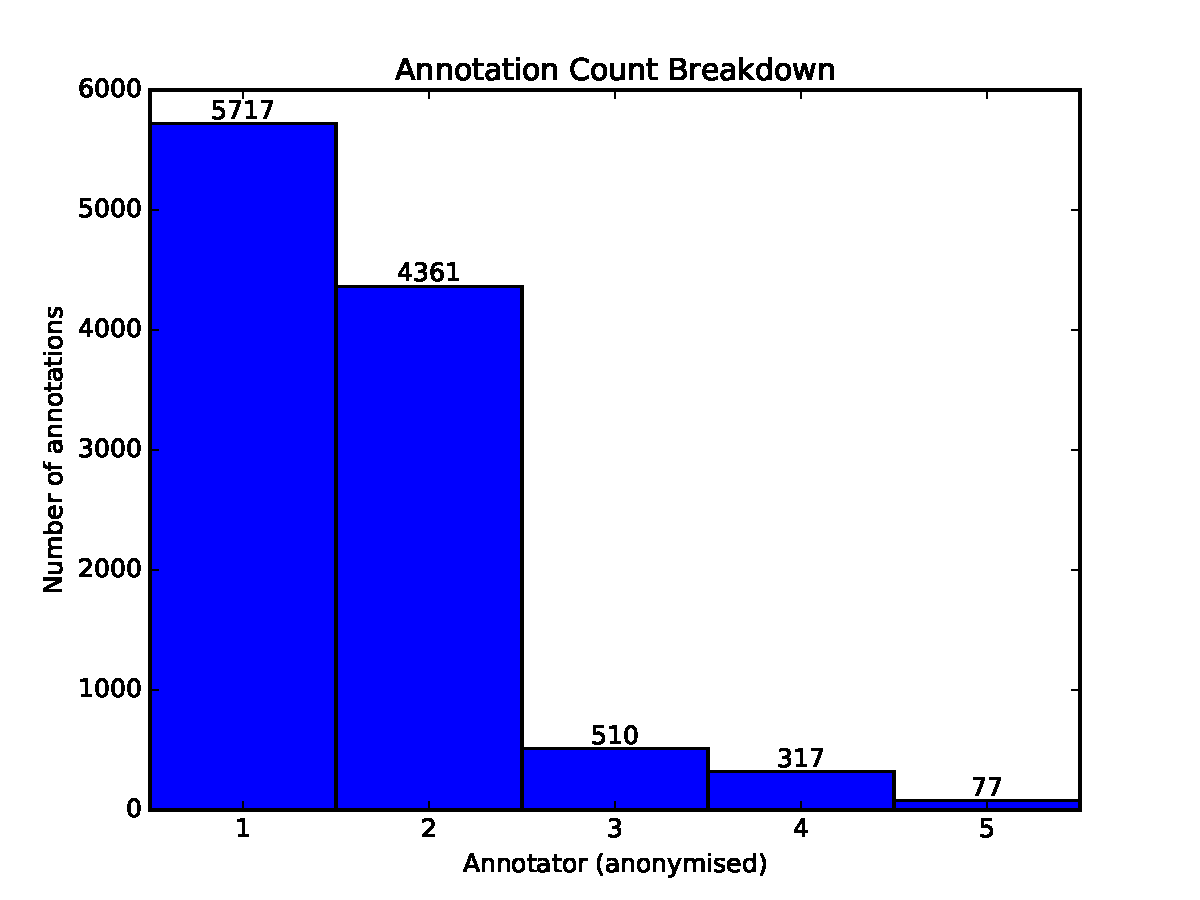
\includegraphics[width=0.95\textwidth]{graphs/annotator-breakdown}
    \caption{Total number of annotations by annotator}
    \label{fig:annotator-breakdown}
\end{figure}

In total, five annotators managed to annotate a total of 10,982 images across all annotation methodologies. Figure \ref{fig:annotator-breakdown} illustrates the number of annotations completed by each annotator. Two annotators accounted for the majority of the annotations, while three others provide an additional 904. The exact number of each annotation type, the total time it took to annotate each annotation type and the average time it took to annotate is displayed in Table \ref{table:annotation-stats}.

\begin{table}[ht]
    \centering
    \begin{tabular}{ | l | l | l | l | p{5cm} |}
    \hline
    Name & Count & Average Time & Total Time \\ \hline
    Text & 3172 & 1 minute & 2 days, 23 hours \\ \hline
    Tag & 2897 & 31 seconds & 23 hours, 40 minutes \\ \hline
    Query & 3616 & 16 seconds & 15 hours, 10 minutes \\ \hline
    Assessment & 1327 & 58 seconds & 21 hours, 36 minutes \\ \hline
    \end{tabular}
    \caption{Annotation Statistics}
    \label{table:annotation-stats}
\end{table}

\begin{figure}[ht]
    \centering
    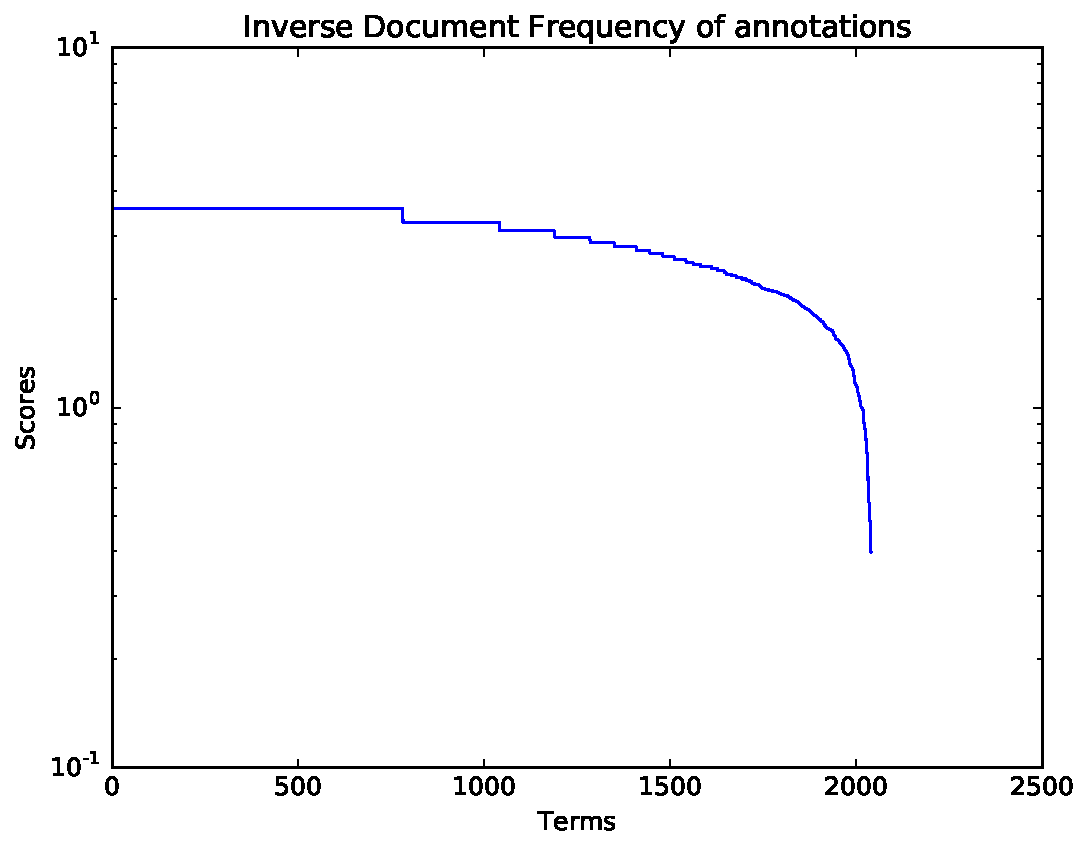
\includegraphics[width=0.7\textwidth]{graphs/idf-scores}
    \caption{IDF scores for concepts in the annotations}
    \label{fig:idf-scores}
\end{figure}

\begin{figure}[ht]
    \centering
    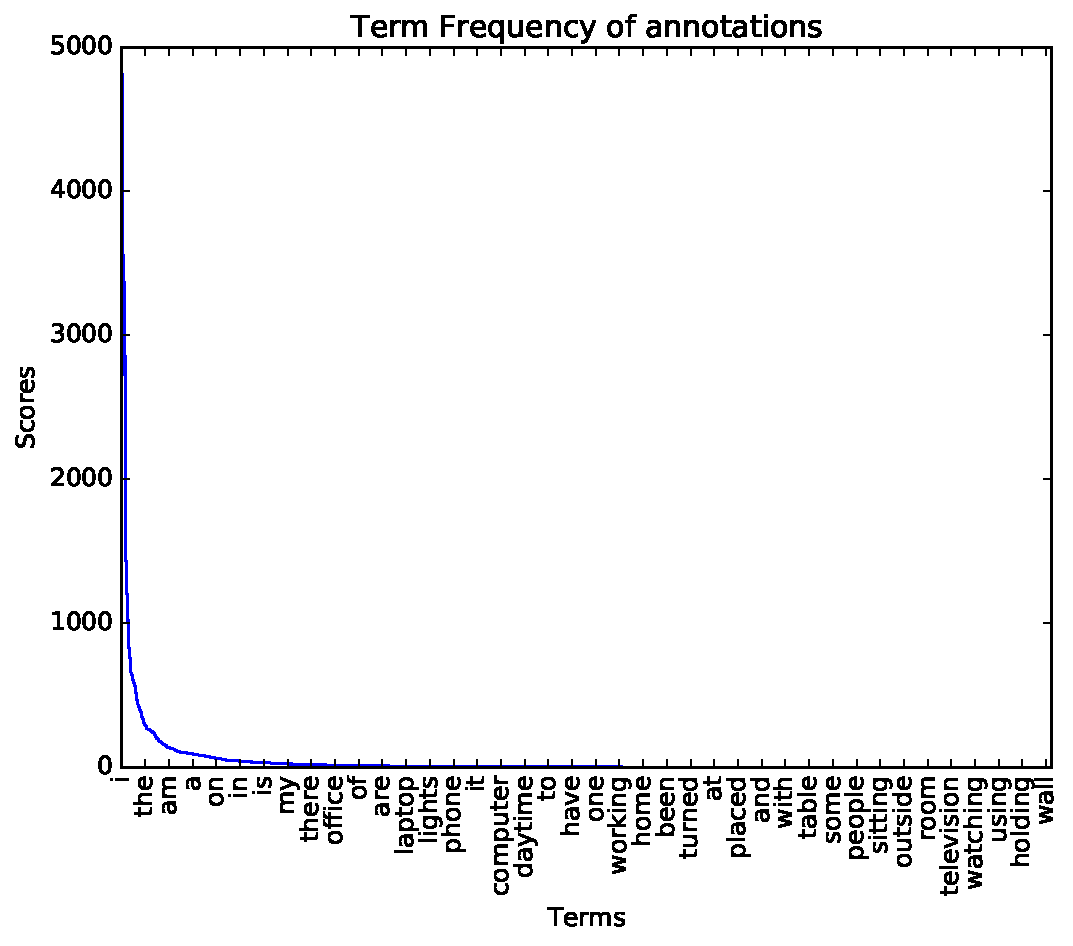
\includegraphics[width=0.7\textwidth]{graphs/tf-scores}
    \caption{Term Frequency scores for concepts in the annotations}
    \label{fig:tf-scores}
\end{figure}

Textual annotations accounted for the highest amount of time taken on average in the collection process. The largest number of annotations collected for a methodology are the query annotations. Accounts from annotators note that the relevance assessments are the most tedious to collect. Explaining the time it takes to annotate images each methodology is somewhat intuitive -- formulating a query for a typical commercial search engine does not take a very long time, which can account for the marginal average time for this annotation type. On the other hand, composing (in the annotators mind and physically typing on a keyboard) a descriptive paragraph filled with context and semantics naturally leads to the conclusion that textual annotations do, in fact, take a significant amount of time to annotate. Secondly, the process of completing a relevance assessment involves scrolling and clicking a multitude of times; this time adds up and is evident in the average time.

\FloatBarrier
\section{Retrieval Effectiveness}

Each experiment is displayed as a table which provides the results from \verb|trec_eval| and as a precision-recall graph. The results from only the manually annotated images are displayed first. Table \ref{table:manual-results-title} presents the \verb|trec_eval| results for the four annotation methodologies \textit{and} the result of combining all four of the methodologies. These results are visualised as a precision-recall graph in Figure \ref{fig:manual-result-title}. The query annotations retrieve the most images, however when combining all four collections of annotations together the scores all increase slightly, and a reciprocal rank of $1.0$ is achieved.

\begin{table}[ht]
    \centering
    \begin{tabular}{|c|c|c|c|c|}
        \hline
         Methodology & MAP & RR & P@10 & Relevant Retrieved \\ \hline
         Text & 0.3442 & 0.9223 & 0.8333 & 1062 \\ \hline
         Tag & 0.5468 & 0.9578 & 0.8396 & 1040 \\ \hline
         Query & 0.6400 & 0.9653 & 0.8750 & 1559 \\ \hline
         Relevance Assessment & 0.4815 & 0.8406 & 0.6917 & 831 \\ \hline
         All & 0.6495 & 1.000 & 0.9062 & 1612 \\ \hline
    \end{tabular}
    \caption{MAP, Reciprocal Rank, and Precision at 10 scores for the manual annotations using titles}
    \label{table:manual-results-title}
\end{table}

\begin{table}[ht]
    \centering
    \begin{tabular}{|c|c|c|c|c|}
        \hline
         Methodology & MAP & RR & P@10 & Relevant Retrieved \\ \hline
         Text & 0.5285 & 0.9792 & 0.8521 & 1088 \\ \hline
         Tag & 0.4627 & 0.8928 & 0.7687 & 1055 \\ \hline
         Query & 0.4457 & 0.7683 & 0.5958 & 1566 \\ \hline
         Relevance Assessment & 0.5219 & 0.9271 & 0.7938 & 972 \\ \hline
         All & 0.5855 & 0.9815 & 0.8875 & 1613 \\ \hline
    \end{tabular}
    \caption{MAP, Reciprocal Rank, and Precision at 10 scores for the manual annotations using descriptions}
    \label{table:manual-results-title}
\end{table}

\begin{figure}[ht]
    \centering
    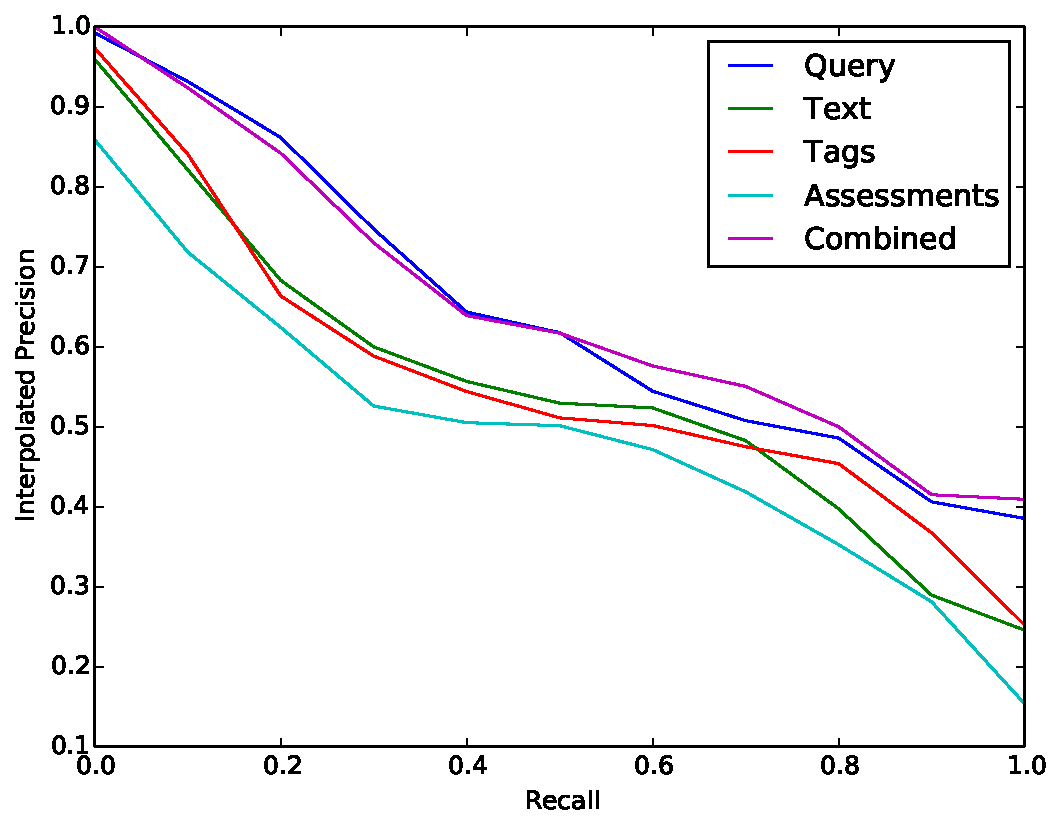
\includegraphics[width=0.8\textwidth]{graphs/manual-title}
    \caption{Precision-recall curves for the manual annotations using topic titles}
    \label{fig:manual-result-title}
\end{figure}

\begin{figure}[ht]
    \centering
    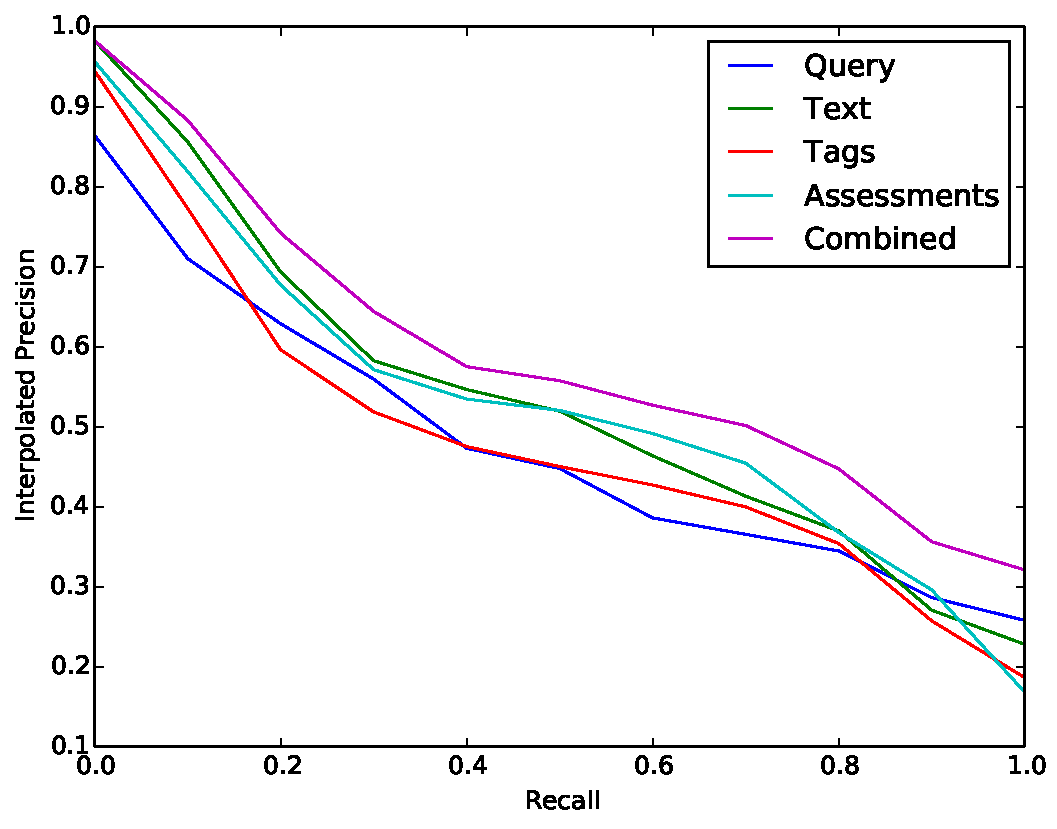
\includegraphics[width=0.8\textwidth]{graphs/manual-desc}
    \caption{Precision-recall curves for the manual annotations using topic descriptions}
    \label{fig:manual-result-desc}
\end{figure}

\FloatBarrier

A neuraltalk2 is trained on the manual textual, tag, and query annotations (i.e after the manual annotates are collected). The neural network architecture is able to produce captions for every image in the collection. The quality of these captions is summarised in Table \ref{table:learnt-results} -- clearly not the most impressive results. The automatic captions that are generated are evaluated in the same way as the manual annotations. The output of the neural network is formatted to be used in the evaluation pipeline as described in Section \ref{methods:evaluating}. 

There is no clear individual annotation methodology that outperforms the others, the scores are too low to indicate this. Combining the three automatic annotations together does seem to increase the overall precision. The learnt queries do retrieve the most number of images, in a similar result to the manual annotation results.

The number of iterations the neural network covered for each annotation methodology is visualised in Figures \ref{fig:val-loss-1} and \ref{fig:val-loss-2}. The results of the automatic captioning do not get better over time --- in fact they get worse. This is a concerning finding, and it can most likely be attributed the the lack of training examples. The gap between topics with a large number of relevant images and the number of training examples in combination with topics that contain a very low number of relevant images is presumably the contributing factor to these graphs.

\begin{table}[ht]
    \centering
    \begin{tabular}{|c|c|c|c|c|}
        \hline
         Methodology & MAP & RR & P@10 & Relevant Retrieved\\ \hline
         Text & 0.0048 & 0.0248 & 0.0196 & 187 \\ \hline
         Tag & 0.0083 & 0.0184 & 0.0022 & 136 \\ \hline
         Query & 0.0076 & 0.0174 & 0.0021 & 246 \\ \hline
         All & 0.0164 & 0.0393 & 0.0169 & 337 \\ \hline
    \end{tabular}
    \caption{MAP, Reciprocal Rank, and Precision at 10 scores for the automatically generated annotations using titles}
    \label{table:learnt-results-title}
\end{table}

\begin{table}[ht]
    \centering
    \begin{tabular}{|c|c|c|c|c|}
        \hline
         Methodology & MAP & RR & P@10 & Relevant Retrieved\\ \hline
         Text & 0.0048 & 0.0232 & 0.0167 & 222 \\ \hline
         Tag & 0.0050 & 0.0184 & 0.0063 & 145 \\ \hline
         Query & 0.0051 & 0.0062 & 0.0062 & 199 \\ \hline
         All & 0.0096 & 0.0470 & 0.0187 & 325 \\ \hline
    \end{tabular}
    \caption{MAP, Reciprocal Rank, and Precision at 10 scores for the automatically generated annotations using descriptions}
    \label{table:learnt-results-title}
\end{table}

\begin{figure}[ht]
    \centering
    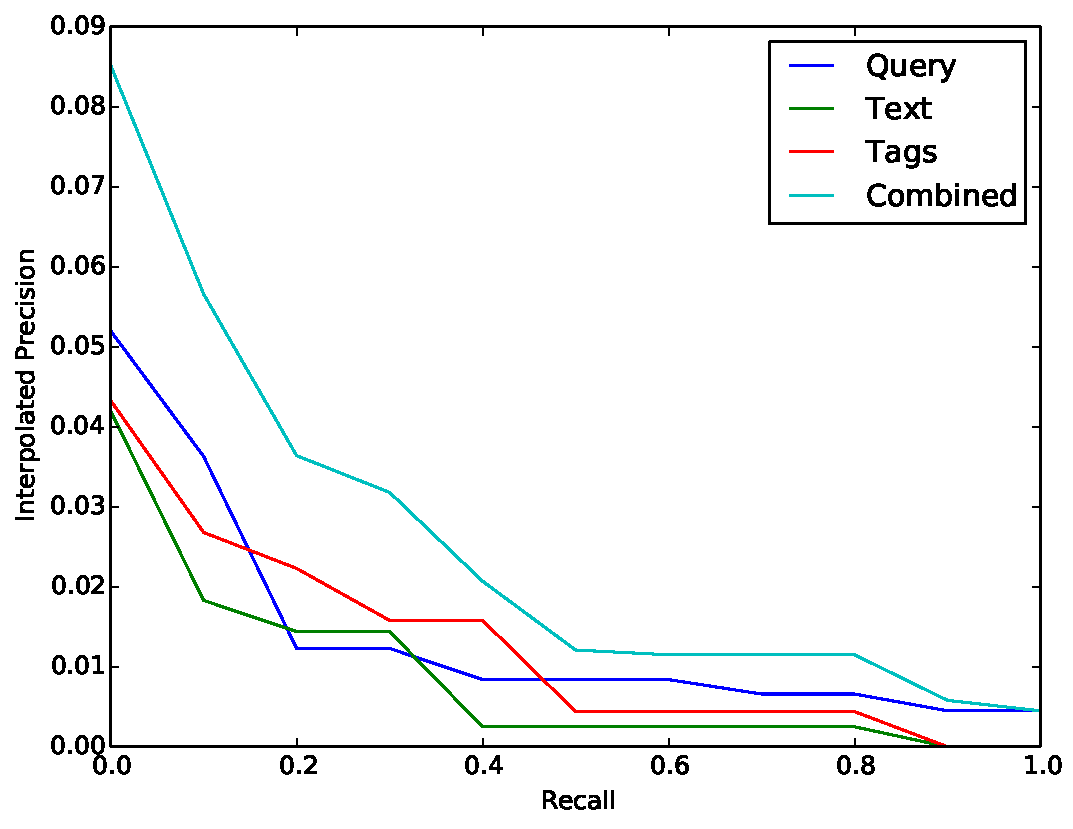
\includegraphics[width=0.8\textwidth]{graphs/auto-title}
    \caption{Precision-recall curves for the learnt annotations using titles}
    \label{fig:manual-result-title}
\end{figure}

\begin{figure}[ht]
    \centering
    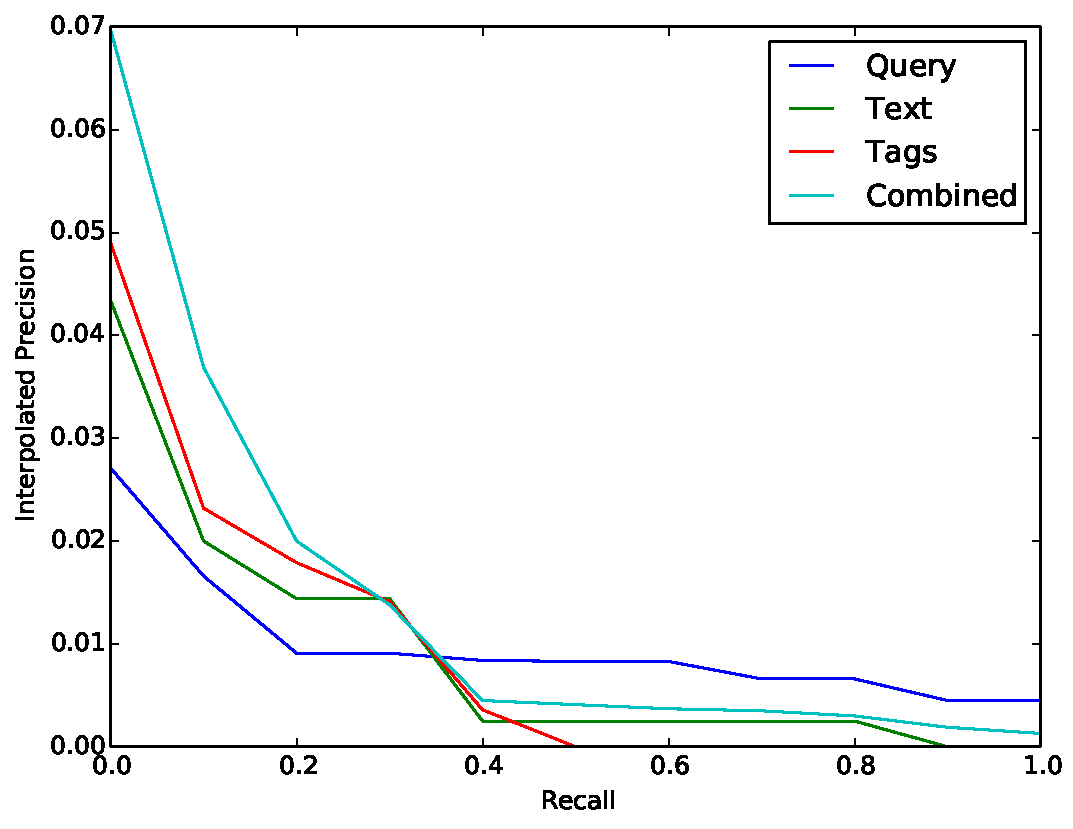
\includegraphics[width=0.8\textwidth]{graphs/auto-desc}
    \caption{Precision-recall curves for the learnt annotations using descriptions}
    \label{fig:manual-result-desc}
\end{figure}

\begin{figure}
    \centering
    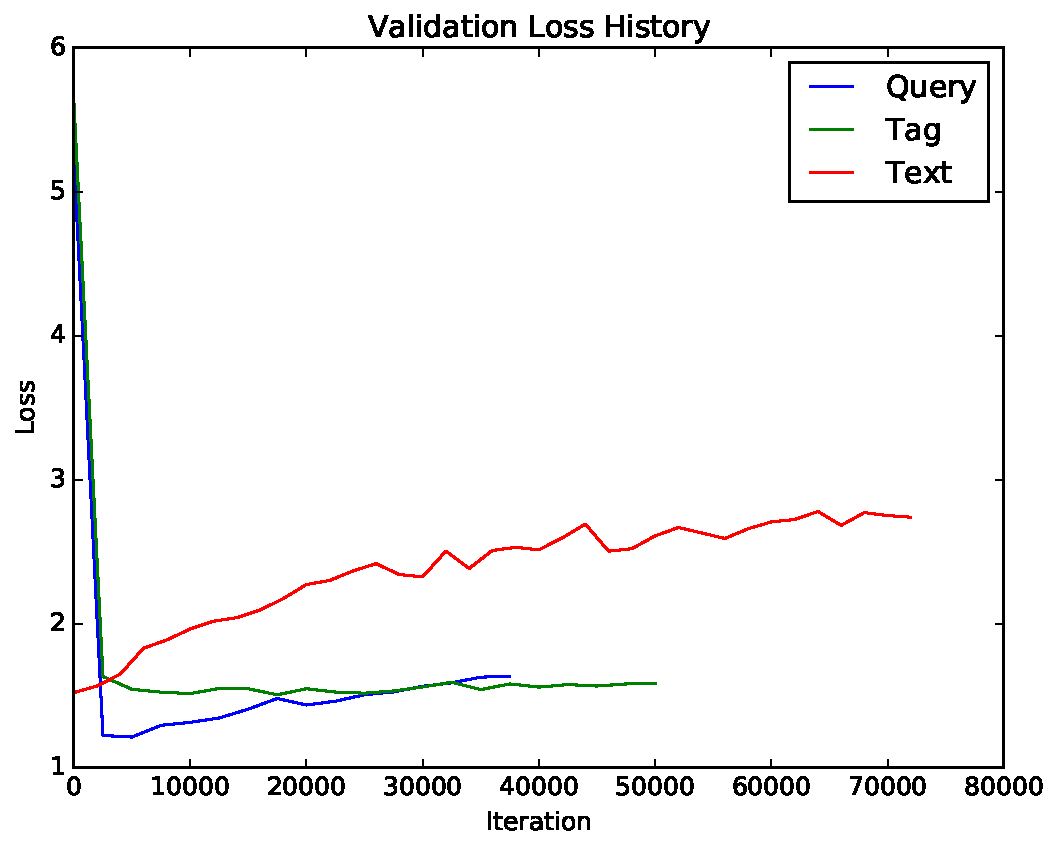
\includegraphics[width=0.7\textwidth]{graphs/initial-validation-loss-history}
    \caption{Validation loss history (\textless 100,000 iterations)}
    \label{fig:val-loss-1}
\end{figure}

\begin{figure}
    \centering
    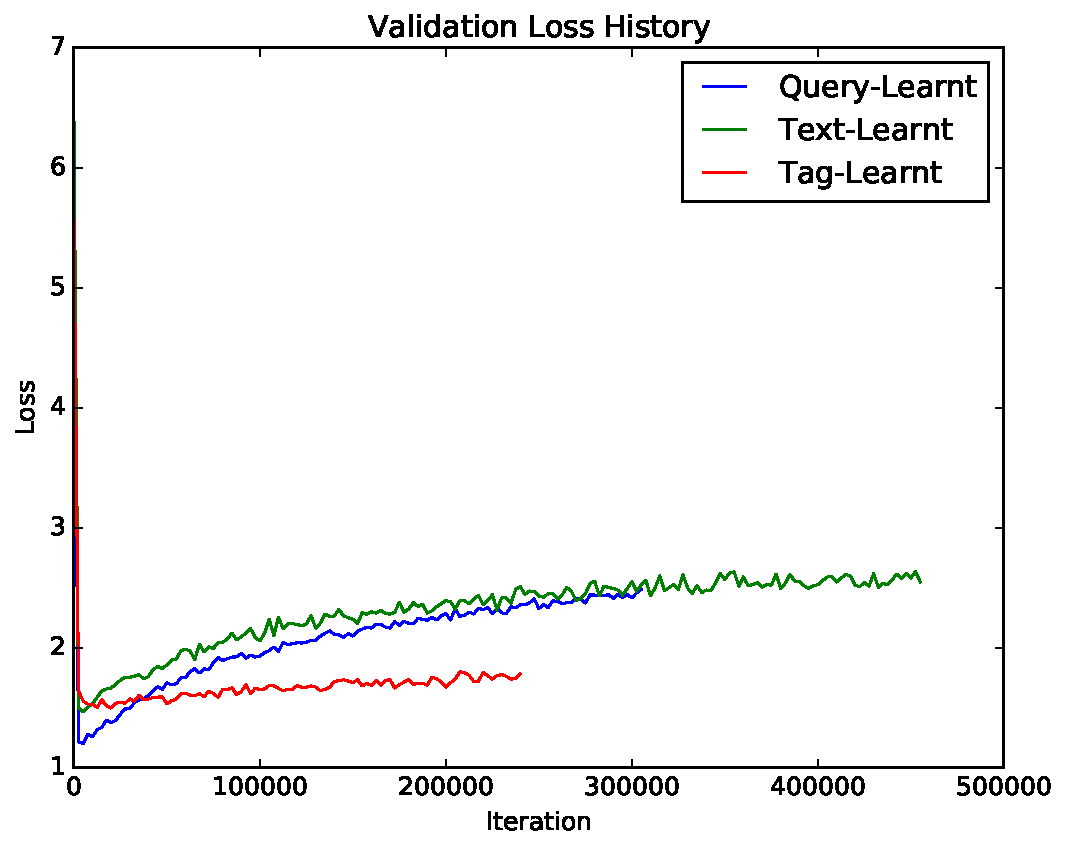
\includegraphics[width=0.7\textwidth]{graphs/validation-loss-history}
    \caption{Validation loss history (\textgreater 200,000 iterations)}
    \label{fig:val-loss-2}
\end{figure}